\documentclass[aps,prl,reprint,groupedaddress,superscriptaddress]{revtex4-2}

\usepackage{amsmath}
\usepackage{amssymb}
\usepackage{graphicx}
\usepackage{hyperref}
\hypersetup{colorlinks=true,urlcolor=blue,linkcolor=black,citecolor=black}

\begin{document}

\title{The Levitron Lab: Interactive Teaching of Magnetic Levitation Across Feedback, Gyroscopic, and Driven-Rotation Regimes}

\author{Saleem Aldajani}
\affiliation{Massachusetts Institute of Technology, Cambridge, Massachusetts 02139, USA}
\email{saldajani@mit.edu}

\date{\today}

\begin{abstract}
Earnshaw's theorem forbids stable levitation in static fields, yet familiar tabletop toys appear to violate it. We present \emph{The Levitron Lab}, an open-source browser suite of five interactive simulations ordered by the dimensionality of the instability each device must overcome. Each module integrates governing equations in real time, exposes every parameter through interactive controls, displays potential landscapes and Jacobian eigenvalues, and foregrounds a live rendering of the levitating body. The gyroscopic module implements the symmetric-top nutation analysis of the author's prior MIT 8.223 project, including the restoring potential $U_{\mathrm{res}}(\theta)$ and bounded nutation window. Source: \url{https://github.com/saldajani/levitron-lab}.
\end{abstract}

\maketitle

\begin{figure}[t]
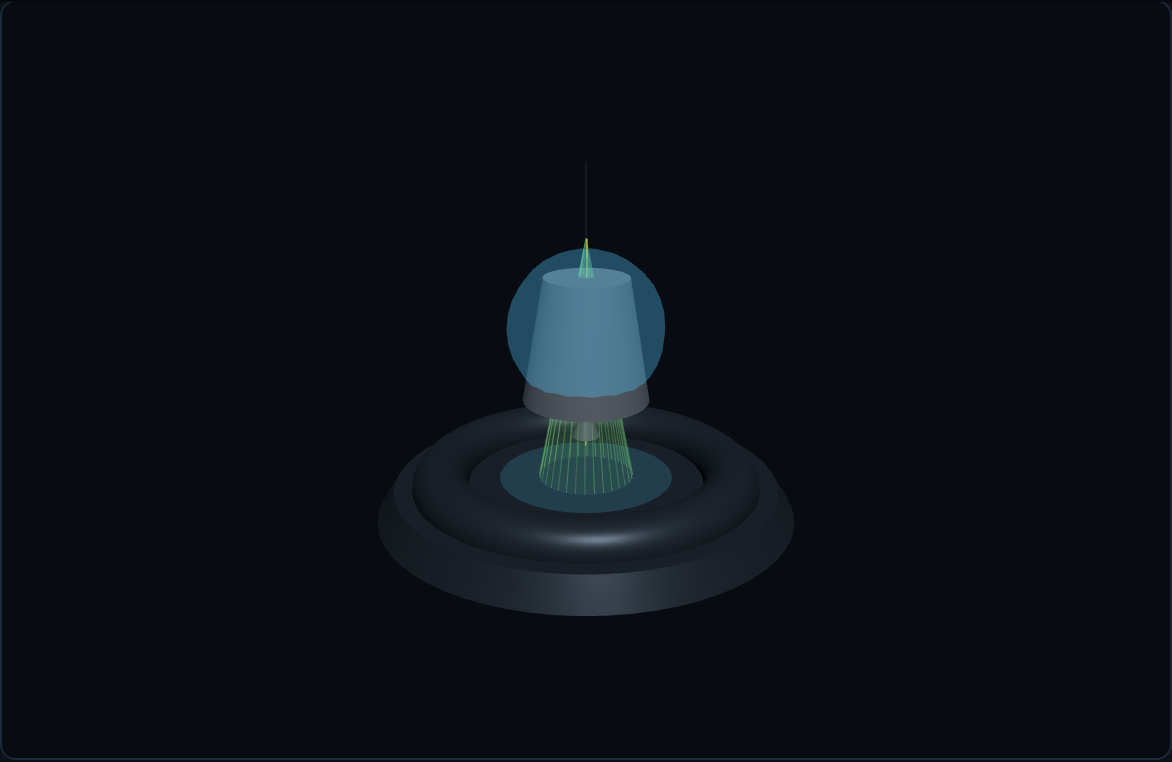
\includegraphics[width=\linewidth]{figures/fig_gyro_stable.png}
\caption{\label{fig:gyro}Module~3: gyroscopic Levitron at the default stable preset, showing the spinning top, symmetry axis, and allowable nutation cone (half-angle $\theta_c$).}
\end{figure}

\textit{Introduction.}---Static equilibrium of a magnetic dipole is a saddle (Earnshaw). Commercial levitators escape via active feedback, gyroscopic spin, or driven rotation~\cite{simon,berry}. We unify all three in one curriculum climbing from one-dimensional to full six-degree-of-freedom dynamics, motivated by the observation that the classic Levitron is a macroscopic magnetic atom trap~\cite{ketterle}.

\textit{Architecture.}---Client-side React/TypeScript/\texttt{three.js}; fixed-step integration (semi-implicit Euler for feedback; RK4 for rigid-body modules); live Jacobian eigenvalues in feedback modules (Fig.~\ref{fig:eigs1d}).

\begin{figure}[t]
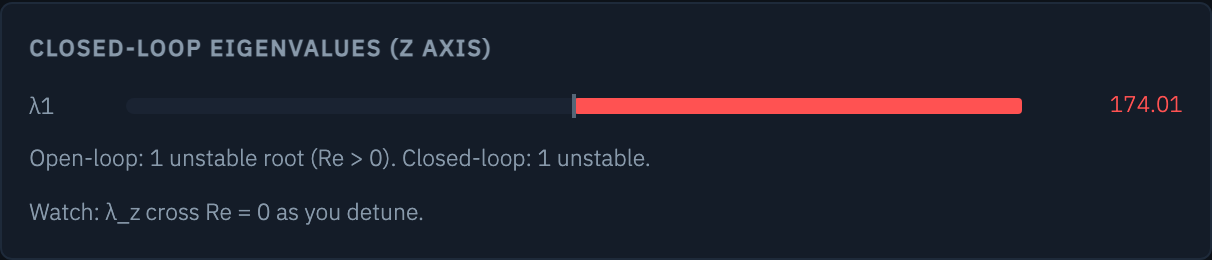
\includegraphics[width=0.48\linewidth]{figures/fig_feedback1d_eigs.png}
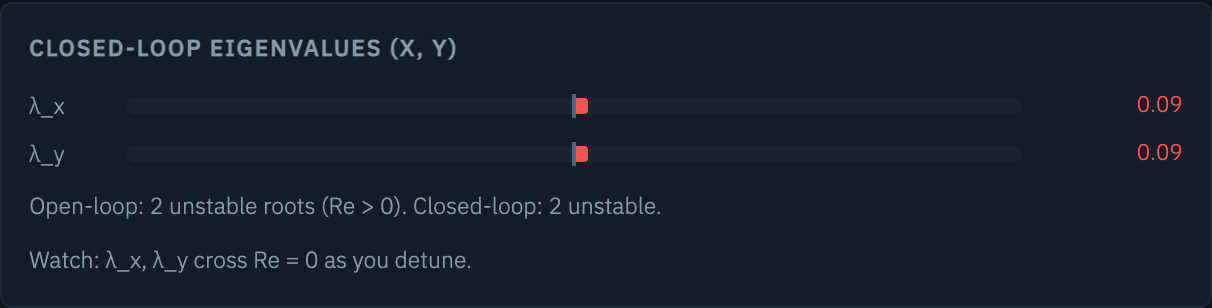
\includegraphics[width=0.48\linewidth]{figures/fig_feedback2d_eigs.png}
\caption{\label{fig:eigs1d}Closed-loop eigenvalues: Module~1 (unstable $z$ open-loop) vs.\ Module~2 (unstable $x,y$).}
\end{figure}

\textit{Gyroscopic module.}---Following Aldajani \& Alowayed~\cite{aldajani823}, we use Euler angles $(\varphi,\theta,\psi)$ with conserved momenta $p_\psi=I_s(\dot\psi+\dot\varphi\cos\theta)$ and $p_\varphi=(I_p\sin^2\theta+I_s\cos^2\theta)\dot\varphi+I_s\dot\psi\cos\theta$. Nutation obeys the effective potential
\begin{equation}
U_{\mathrm{res}}(\theta)=\frac{p_\psi^2}{2I_s}+\frac{(p_\varphi-p_\psi\cos\theta)^2}{2I_p\sin^2\theta}+V_{\mathrm{eff}}(\theta),
\end{equation}
with slow-precession launch $\dot\varphi=mgl/p_\psi$ and bounded nutation $\theta_{\min}<\theta<\theta_{\max}$ (Fig.~\ref{fig:ures}). Stability requires both the spin window and this nutation cone.

\begin{figure}[t] 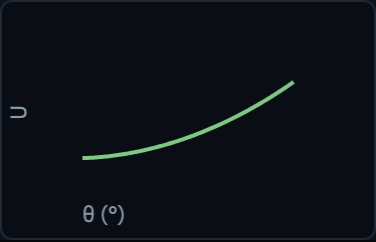
\includegraphics[width=\linewidth]{figures/fig_gyro_potential.png} \caption{\label{fig:ures}$U_{\mathrm{res}}(\theta)$ well with $\theta_c$ annotation; bounded nutation between turning points.} \end{figure}

\textit{Dynamical rotor.}---Motor-driven rotor traps a floater via frequency lock~\cite{hermansen,doff} (Fig.~\ref{fig:rotor}).

\begin{figure}[t] 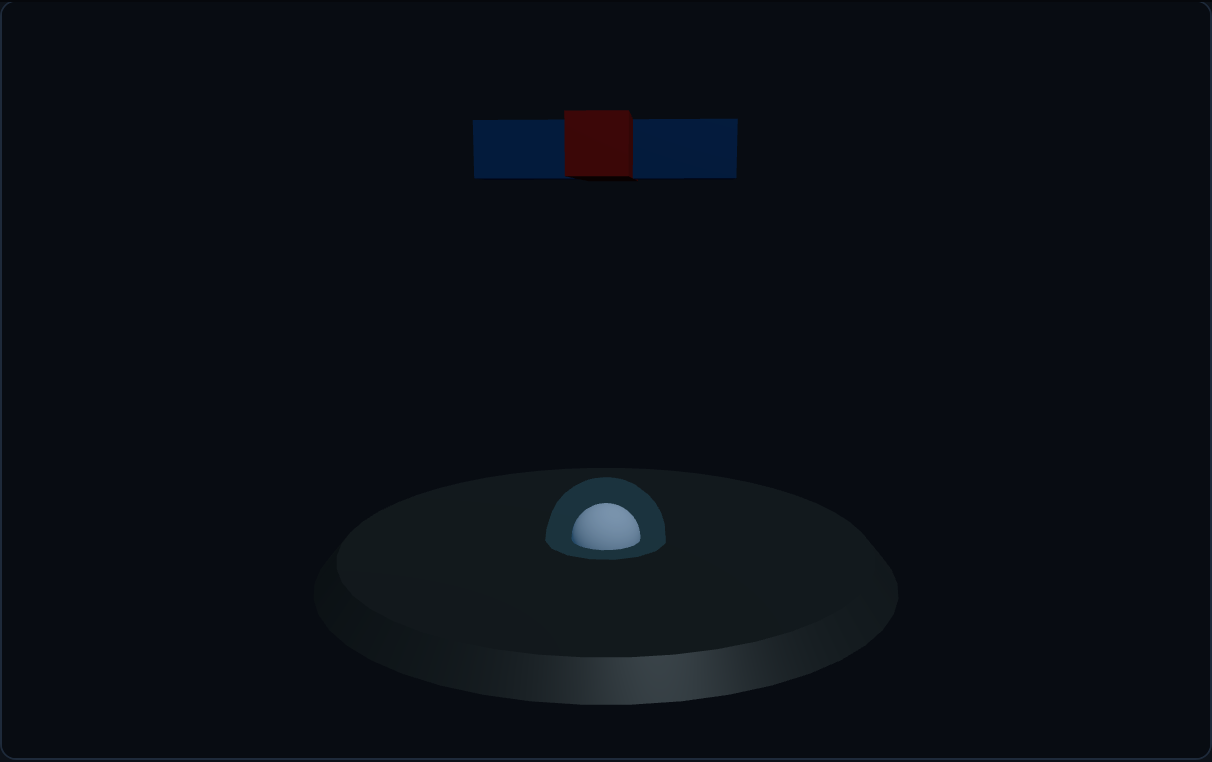
\includegraphics[width=\linewidth]{figures/fig_rotor_trap.png} \caption{\label{fig:rotor}Module~4: rotor and frequency-locked floater below.} \end{figure}

\textit{Availability.}---\url{https://github.com/saldajani/levitron-lab}; one-click GitHub Codespaces; video~\cite{video}.

\begin{acknowledgments}
Thanks to W.~Ketterle for the atom-trap analogy~\cite{ketterle}.
\end{acknowledgments}

\begin{thebibliography}{99}
\bibitem{aldajani823} S.~Aldajani and Alowayed, ``Understanding the Levitron Through the Analysis of a Symmetric Spinning Top in a Gravitational Field,'' MIT 8.223 project (author's prior work). \url{http://goo.gl/c5u3lk}
\bibitem{video} S.~Aldajani, Levitron analysis video. \url{https://www.youtube.com/watch?v=1LHwq_g06fE}
\bibitem{simon} M.~D.~Simon \textit{et al.}, Am.\ J.\ Phys.\ \textbf{65}, 286 (1997).
\bibitem{berry} M.~V.~Berry, Proc.\ R.\ Soc.\ Lond.\ A \textbf{452}, 1207 (1996).
\bibitem{hermansen} J.~M.~Hermansen \textit{et al.}, Phys.\ Rev.\ Applied \textbf{20}, 044036 (2023).
\bibitem{doff} A.~Doff and R.~M.~Szmoski, arXiv:2506.23268.
\bibitem{apsfocus} R.~Berkowitz, Physics (APS) \textbf{16}, 177 (2023).
\bibitem{mitviz} MIT VIZ Group. \url{https://web.mit.edu/viz/levitron/Physics.html}
\bibitem{wiki} Wikipedia, spin-stabilized magnetic levitation.
\bibitem{ketterle} W.~Ketterle, personal communication, MIT, June 2026.
\end{thebibliography}

\end{document}
